\documentclass[twoside,11pt]{article}

% Any additional packages needed should be included after jmlr2e.
% Note that jmlr2e.sty includes epsfig, amssymb, natbib and graphicx,
% and defines many common macros, such as 'proof' and 'example'.
%
% It also sets the bibliographystyle to plainnat; for more information on
% natbib citation styles, see the natbib documentation, a copy of which
% is archived at http://www.jmlr.org/format/natbib.pdf

\usepackage{jmlr2e}
\usepackage{graphicx}
\graphicspath{ {images/} }



\begin{document}

\title{Research Paper: Machine Learning Application for Brain Tumor Localization in the  Repository of Molecular Brain Neoplasia Data (REMBRANDT) }

\maketitle
\textbf{Machine Learning for Health Care (Heinz 95-845) - Lukas Mohs}


\section{Abstract}
\noindent Within this paper, I want to present the putcome of the  combined application of \textit{Computer Vision} (CV) and  \textit{Machine Learning} (ML) to the \textit{Repository of Molecular Brain Neoplasia Data } (REMBRANDT) dataset. This dataset contains pre-surgical \textit{magnetic resonance} (MR) multi-sequence images of 130 patients. Based on a visual analysis and the application of several ML algorithms, I tried to predict the location of the brain tumor and compare it to the evaluation of three Radiologist, which defined the affected brain part and the potential impact on the brain functionality.i

\section{Introduction}
\subsection{Brain Cancer}
Among all types of cancer, brain cancer is one of the deadliest even if it's not one of the most common ones. With a so-called \textit{5-Year Relative Survival Rate} of 32 \% for white people and 39 \% for black people it ranks on place 7 out of 26 for the lowest survival rate. Specific cancer types like \textit{Glioblastoma}, a very fast growing type of tumor, even has a a rate of 5\%. Especially in the later years of life, this rate decreases heavily for all types of brain cancer. \citep{cite1}
The high variance in the surivial rate is given by many factors such as the type of tumor, the location and of course whether it was treated. Especially the latter ones formed a major part of scientific studies that included ways of scanning the human brain for malignant tissue as well as the way of stopping the growth of the tumor cells.


\subsection{Magnetic Resonance Imaging (MRI)}
\textit{Magnetic Resonance Imaging} (MRI) addressed the challange of 
\textit{scanning} the human body by using \textit{radiology}  to see different layers of the inner tissue or organs. These different layers can be combined together to construct a 3-dimensional model of any part of the body. Mainly a strong  \textit{magnetic fields} is used in combination with \textit{radio waves}  and so-called \textit{field gradients}.
In comparison to \textit{Computer Tomography} (CT), MRI doesn't rely on \textit{X-radiation}, which qualifies it as a less harmful method. It should be mentioned that the magnetic waves of MRI can affect \textit{cardiac pacemakers} so that exceptions apply. \citep{edelman1993magnetic}

\subsection{The Human Brain}
Especially the development and refinement of the MRI technology favored advanced studies about the structure and functionality of the human brain. In order to understand the classification task of the presented algorithm, the major parts of the human brain are shortly described:
\begin{figure}{\textwidth}
	\centering
	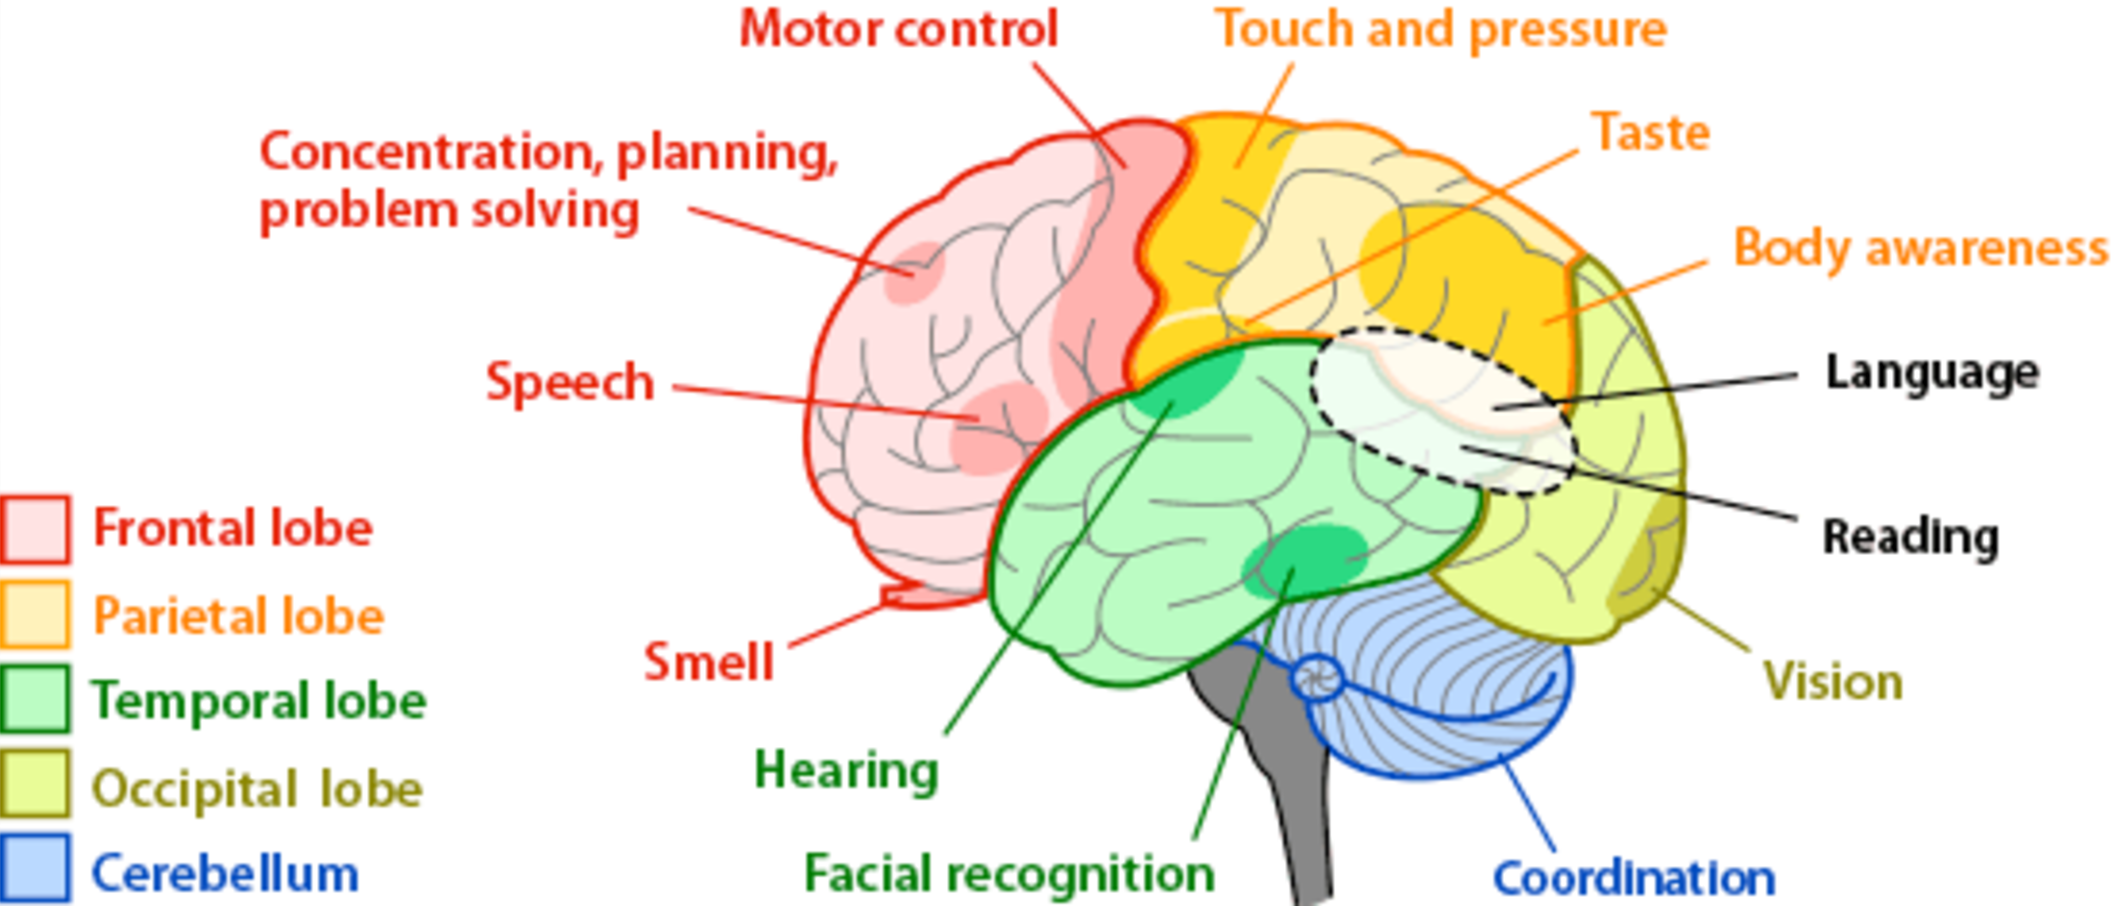
\includegraphics[width=10cm]{brain-areas}
	\caption{Brain Areas (source: Arizona State University)}
\end{figure}%

\begin{itemize}
	\item \textit{Frontal Lobe:} resides in the front of the head and is the only lobe on the lateral surface and separated from the other ones. It is responsible for problem solving, planning but also processes stimuli from the nose. 
	\item \textit{Temporal Lobe:} caudally joins the parietal and occipital lobe without a clear boundary. Researchers could show that it hosts the function of recognizing faces.
	\item \textit{Parietal Lobe:} is Clear separated from frontal lobe but merges into temporal and occipital lobe. It is important for the control of the body including the sense of touch.
	\item \textit{Occipital Lobe:} has also no clear coundary to its neighbours (parietal and temporal lobe). The stimuli of the eye are for example processed by this lobe.
\end{itemize}
\citep{duvernoy2012human}


\bibliography{tumorDetection}
%\appendix
%\section*{Appendix A.}
%Some more details about those methods, so we can actually reproduce them.

\end{document}
